\documentclass[../main.tex]{subfiles}


\begin{document}

\raggedright
The implementation process began with re-constructing the HTML template by Creative Tim\cite{creativeTimTemplate} to the different sections mentioned in chapter 4.2, JavaScript going along with the HTML and finally the Django backend.

\subsection{HTML}
Redesigning the HTML code required changing the CSS, HTML components and removing unwanted JavaScript code. This brought about various bugs and unexpected changes in the overall HTML which crashed a few elements of the code such as Tables. With the use of Google Chrome Console, the debugging was completed and successful HTML pages were created for all three different sections as mentioned in Chapter \ref{ch:design}. However, since pages are going to be repeated(Dashboard, Viewform, Profile, and others), only one HTML code was required and repeated depending on which panel the user logged into. Table \ref{tab:htmlcom} shows what components were created into their related files by redesigning the public licensed template. Each of these was combined with CSS and JavaScript from Chapter \ref{ch:design}. Figures \ref{fig:dash} and \ref{fig:ctdash} show how the template was redesigned to fit our requirements. 

\begin{figure}[H]
        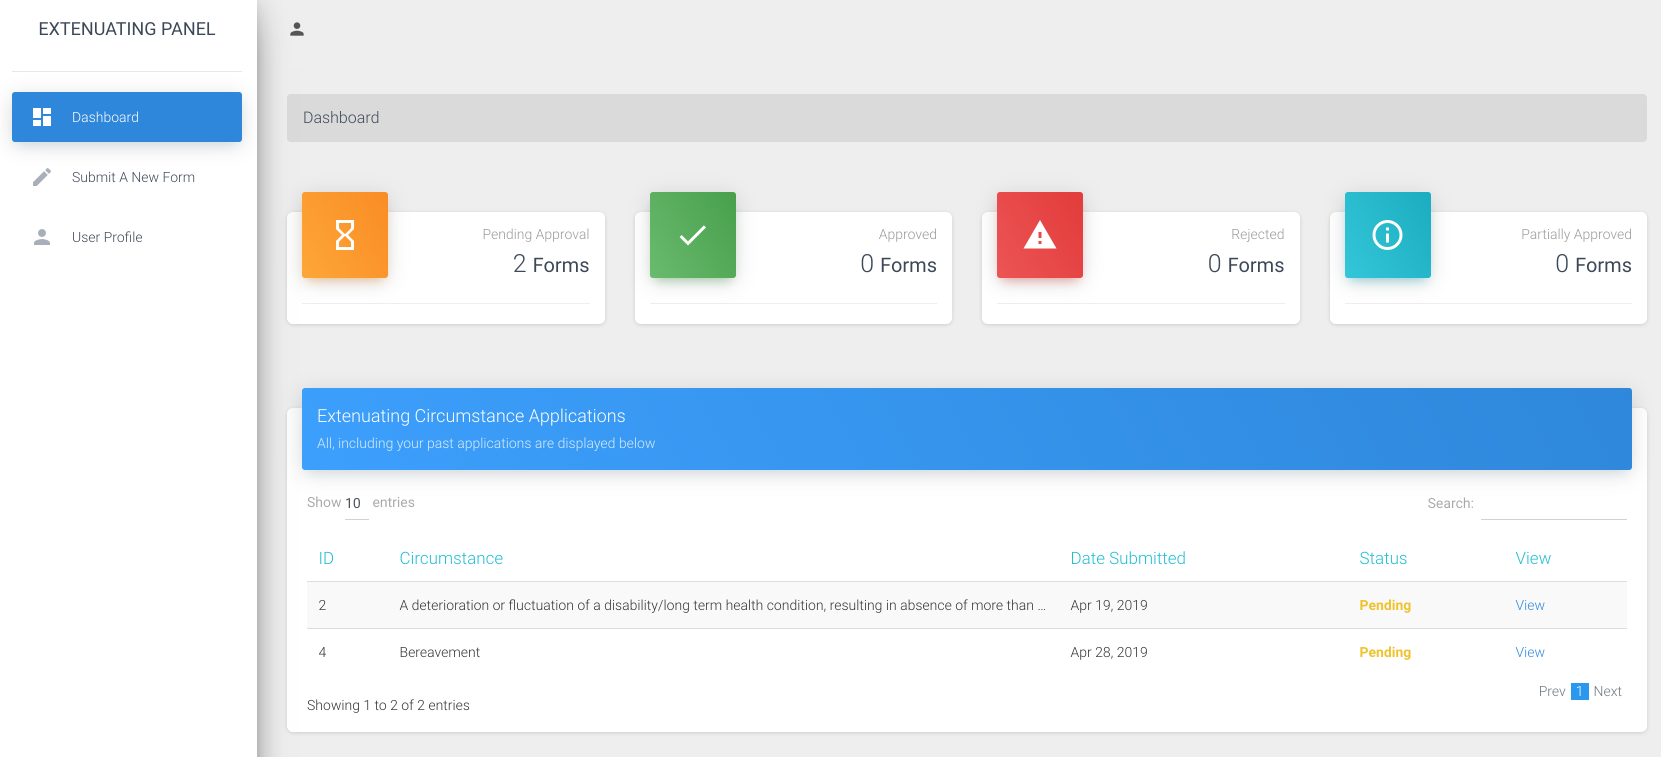
\includegraphics[scale=0.5]
        {images/dash.png}
        \caption{\label{fig:dash} Redesigned Dashboard}
      \end{figure}
      
\begin{figure}[H]
        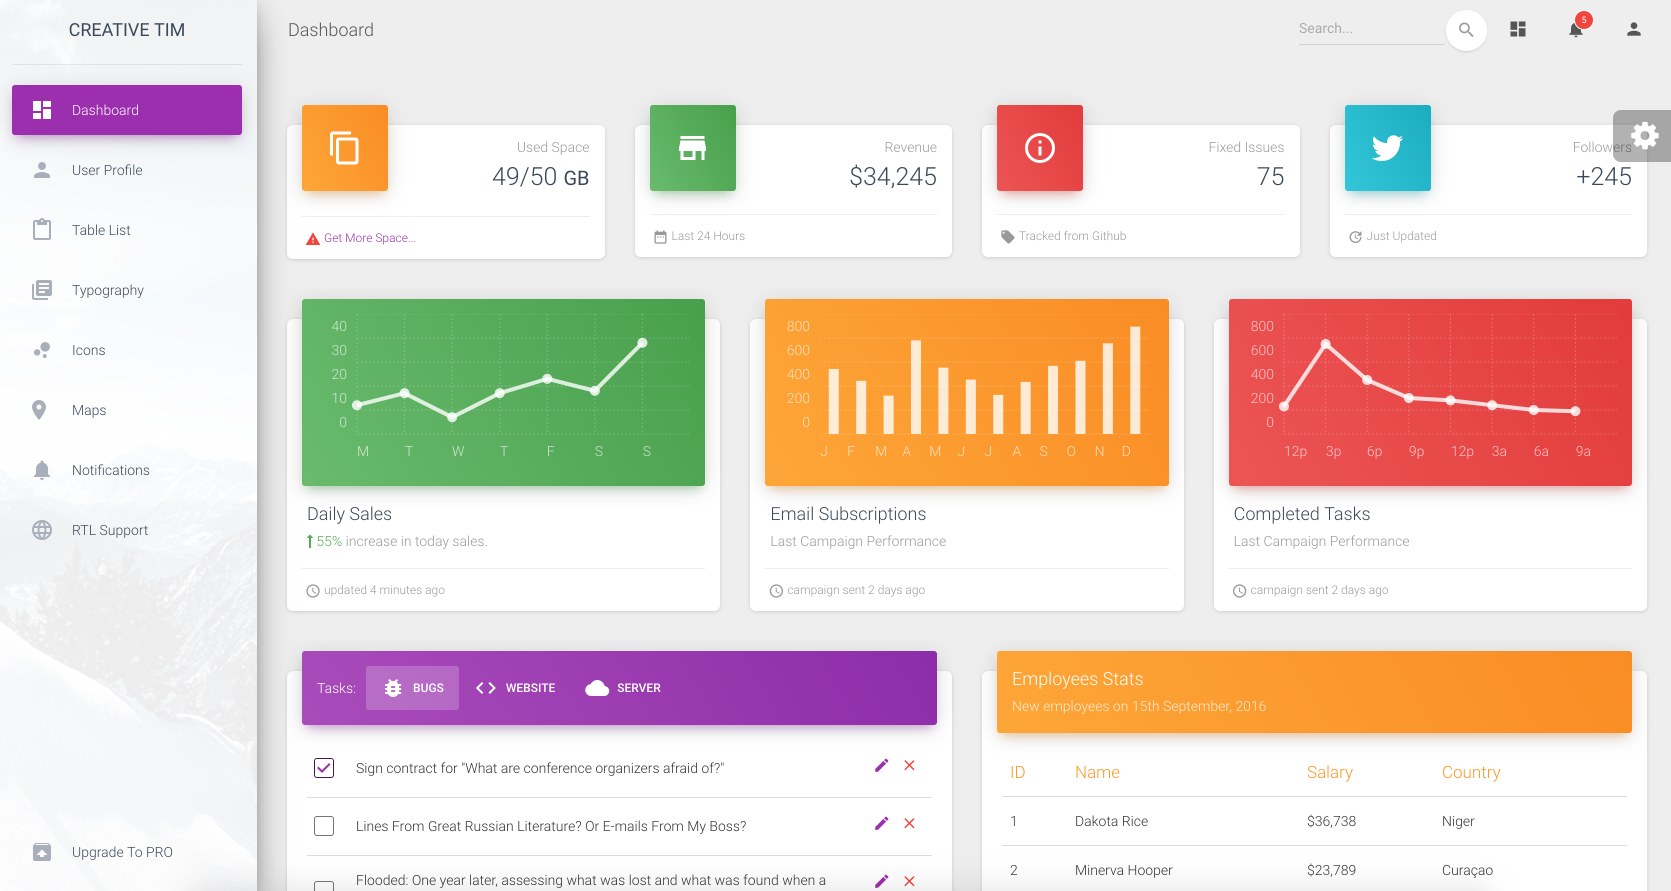
\includegraphics[scale=0.5]
        {images/ctdash.png}
        \caption{\label{fig:ctdash} Creative Tim Dashboard}
      \end{figure}      

\bgroup
\def\arraystretch{2}%  1 is the default, change whatever you need
\begin{table}[H]
\centering
\begin{tabular}{|l| p{9cm} |}
\hline
\textbf{Page} & \textbf{HTML Components} \\ \hline
Login & POST Form(Email, Password) \\ \hline
Register & POST Form(Firstname, Lastname, Email, Password1, Password2, DOB) \\ \hline
Password Change & POST Form(Current Password, Password1, Password2) \\ \hline
Profile Page & POST Form(Email;Disabled, Firstname, Lastname, DOB), TextArea(PublicData) \\ \hline
Dashboard & Statistics, Table(ID, Description, Date, View) \\ \hline
View Form & Text Fields(User Details, Circumstance), Table(Module Details), Table(Uploaded Files), POST Form(Files) \\ \hline
Units & GET Form(Number of modules) \\ \hline
New Form & POST Form(Circumstance, Module Details, Files) \\ \hline
Public Data & TextArea(PublicData;Disabled) \\ \hline
\end{tabular}%
\captionof{table}{HTML Components \&  Relative Pages}\label{tab:htmlcom} 
\end{table}
\egroup

\subsection{JavaScript}
After completion of the HTML design, it was important to add JavaScript in order to allow smooth control of the website. Alongside the JavaScript received with the template by Creative Tim\cite{creativeTimTemplate} such as Bootstrap\cite{bootstrapfour} other scripts were manually added.  \\[4mm]

Tables would load numerous entries for the \textit{Secretary Panel} and the \textit{Scrutiny Panel}, this caused the page to be extensively long without the ability to filter out or search for a specific form, user or find pending forms. In order to achieve efficiency and sort out the entries in the table the use of DataTables\cite{datatables} came in handy. It automatically completed the following;
Added a search field - Allows the user to search for data in the entries\\
Limited entries shown and added more pages - Allows efficiency and speed\\
Sort by ascending or descending - Useful when searching for \textit{Pending} forms \\
Being able to sort and filter through the tables was an important requirement for organised data. \\[4mm]

Another great public script used was \textit{jsPDF}\cite{jsPDF}, as per the requirements, the secretary needs to be able to print and download the forms. PDF would be a perfect format to download these files as any browser, or PDF compatible viewer can be used to view the form. This JavaScript code converts the content inside a specific \textit{HTML container} and copies that data to a PDF which can then be downloaded by the user, in our case, the secretary. When the implementation of this was complete, the data from the form would be saved simply as text and would lose its colours and format. This would scramble up all the data and make it highly unreadable. To overcome this bug, \textit{Html2Canvas} was used. \\[4mm]

\textit{Html2Canvas}\cite{htmlcanvas} is an MIT licensed script which creates an image for everything on the current web page or a specific HTML container with the CSS (including colour and design). This is then copied onto the PDF created by jsPDF as mentioned above and made available for download. This allows the form to be printed the same way it would be seen when viewing it on the web-page. \\[4mm]

Lastly, the secretary can also directly print the form while viewing it. All modern browsers can print directly what is being displayed on the current web page, and with a simple line of code(\textit{window.print()}), a button on the view form HTML allows the browser to detect a print command being sent. 


\subsection{Django}
The main part of the implementation is combining both the HTML and JavaScript to work along with Django being the main controller. In the implementation, Django 2.2\cite{djangoLatest} which is the latest version was used. The first step was to combine the HTML, JavaScript, CSS and Django into a folder system and define it on Django's settings. Within seconds the entire HTML was accessible on a Django running web server. The three sections below explain the process of coding in Django, the difficulties faced and lastly a small summary on back-end development. 

\subsubsection{Authentication \& Database}
After combining all the above, authentication was the first step of coding. As stated in Chapter 4, All-Auth\cite{allauth} was implemented into the Django system by importing the relevant packages. However, in order to avoid users creating multiple accounts with multiple emails, a manual validation was coded which only allows the student's to register with their University Email Address (sheffield.ac.uk) only. All HTML files for All-Auth were overwritten by the HTML design already created in order to have a continuous site. At this point, all data being registered from All-Auth was being stored in an SQLite database which was inbuilt with Django. Creating the database schema, as built-in Chapter \ref{ch:design} seen in \ref{fig:dbschema} was straightforward with the Model, View and Controller system which Django follows. The database was ready in seconds after defining it in Models. Figure \ref{fig:login} and \ref{fig:register} show the login and register pages respectively with All-Auth and Django being the back-end controllers. 


 \begin{figure}[H]
 	\begin{center}
        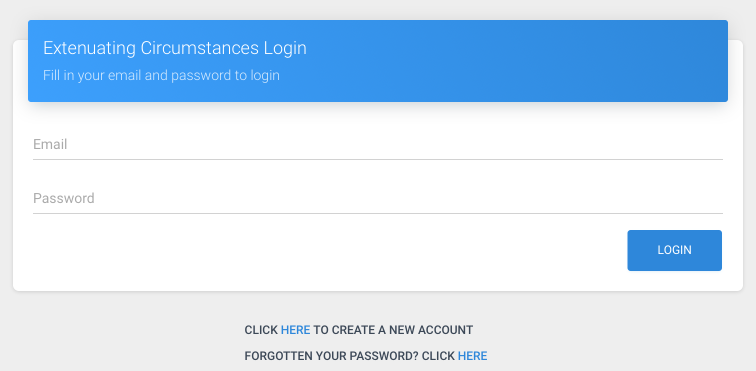
\includegraphics[scale=1]
        {images/login.png}
        \caption{\label{fig:login} Login Page}
     \end{center} 
      \end{figure} 

\begin{figure}[H]
	\begin{center}
        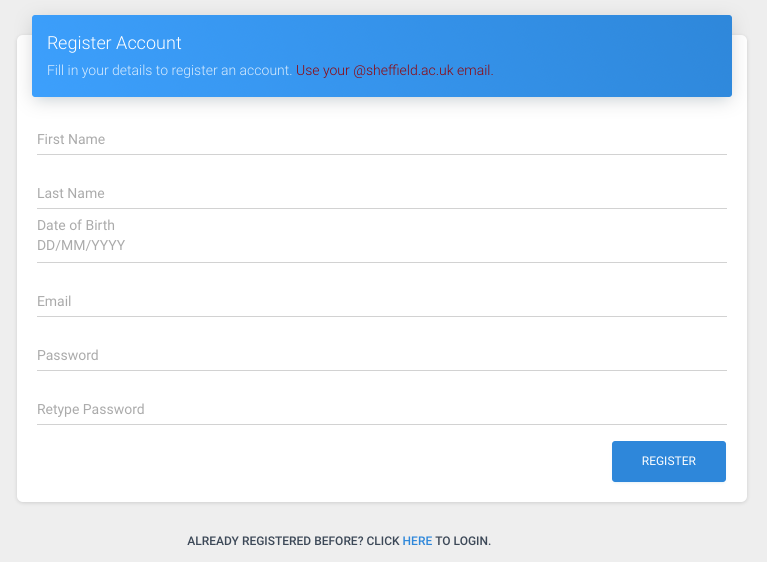
\includegraphics[scale=1]
        {images/register.png}
        \caption{\label{fig:register} Register Page}
     \end{center} 
      \end{figure}
 

\subsubsection{New Form}
At this point, the authentication system was ready as well as the database in which all the data would be stored. In order to retrieve data from the database there needed to be some data already inserted and so in order to do that the "Create a new form" page had to be completed with the back-end code. Different students may have a different number of modules which are affected by their circumstance and so the first step would be to ask them to fill in how many modules are affected by their circumstance. This would send in a GET request with the parameter \textit{units} and its \textit{value} as an integer. The form for creating a new extenuating circumstance would then get this integer from the GET link and produce those many 'input fields' for the modules section of the form. The creation of an HTML POST form is made extremely easy with Django's \textit{forms.py} system where defining the fields of a form such as text input or email automatically present the form on the template where it is called. When the POST data is received, Django runs a \textit{cleaneddata} test which checks for any code in the data received which would be harmful to the system. On successful submit, the student is notified, redirected to dashboard and the form data is saved into the database. The student is also notified if the form was not submitted fully and if it should be re-submitted. Figures \ref{fig:units} and \ref{fig:newform} show the process of creating a new form with the modules from \ref{fig:units} used as a GET request in \ref{fig:newform}

\begin{figure}[H]
        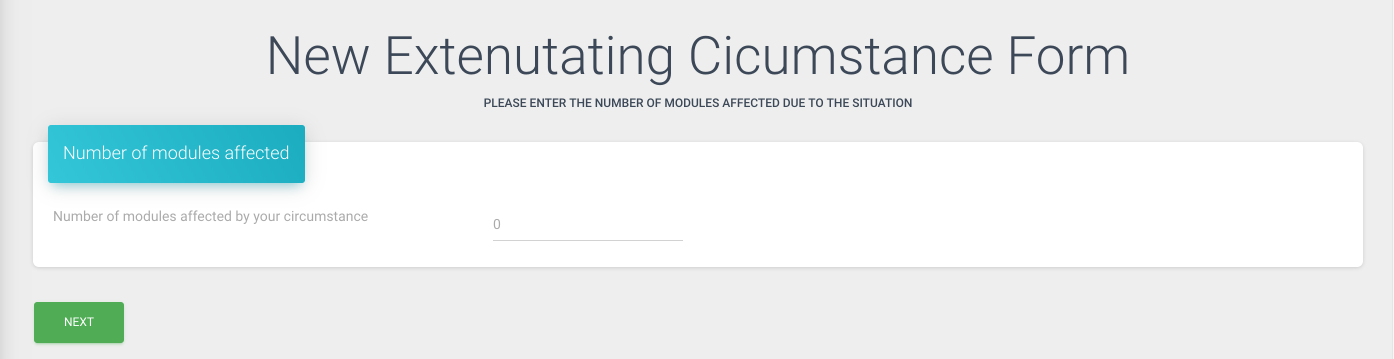
\includegraphics[scale=0.7]
        {images/units.png}
        \caption{\label{fig:units} Number of modules}
      \end{figure}

\begin{figure}[H]
        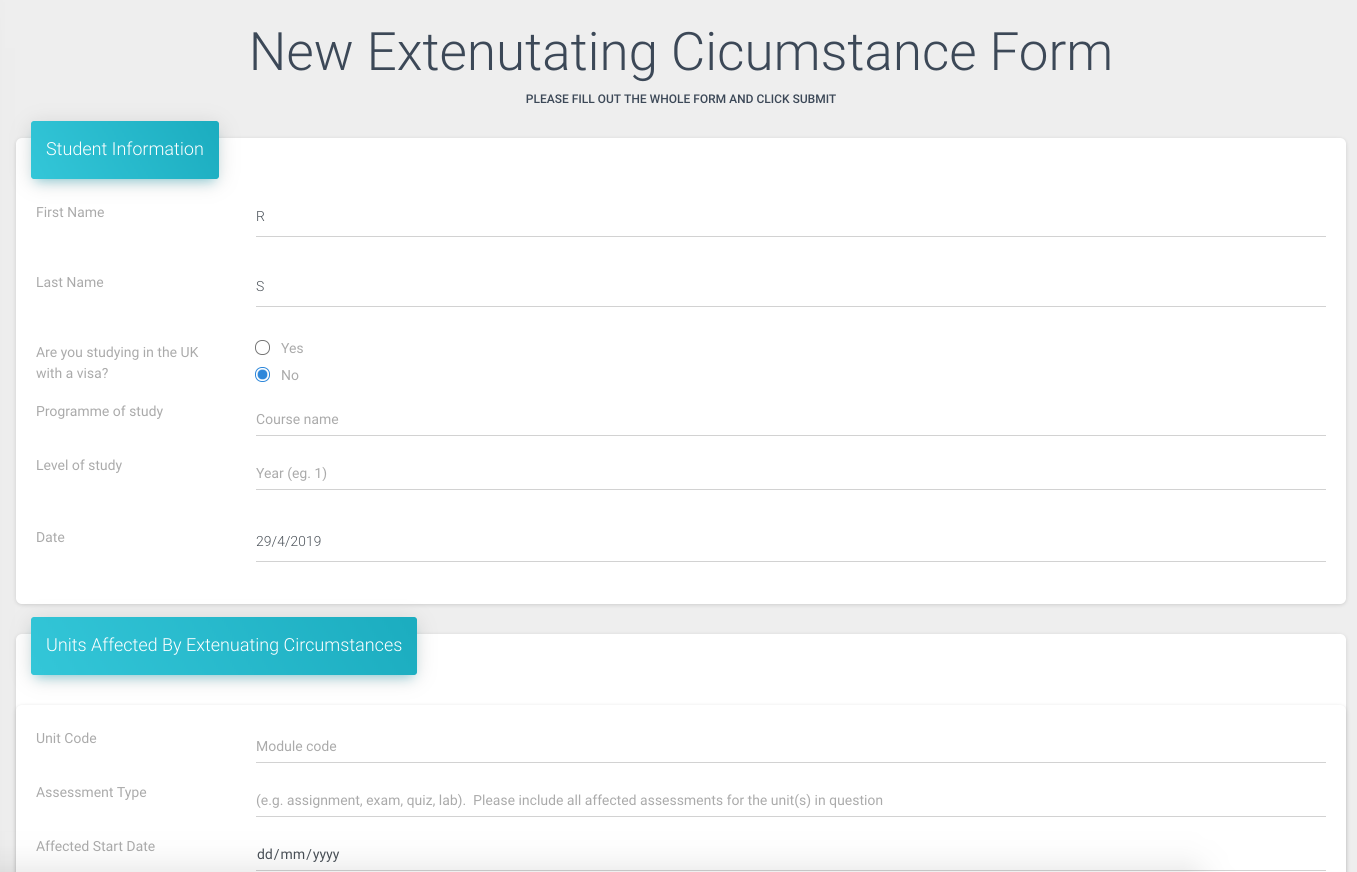
\includegraphics[scale=0.7]
        {images/newform.png}
        \caption{\label{fig:newform} Submit a new form}
      \end{figure}

\subsubsection{Dashboard} 
Student: Once the form has been submitted, the student can see it on the list of forms submitted. The dashboard provides statistics based on the current status of all the forms submitted. These statistics are counted based on the status of each module under each form. If all modules are approved, the form will be entirely approved, and this will be visible to the student under the statistics. The same goes for pending and rejected. However, if the modules are set to different statuses such as \enquote{rejected} and \enquote{approved} under one form, the overall result is \enquote{partially approved} or \enquote{partially pending} if the module has one or more pending modules. The student can see exactly which module has been rejected, approved or still pending.  All data is retrieved from the database and does mathematical calculations where each module is added onto the statistics based on the other modules within the same form. The calculations, as well as the display of each form, was completed easily with the use of \textit{FOR} loops. Figure \ref{fig:dashboardimplement} shows the dashboard created including statistics for the students.\\[4mm] 

Secretary \& Scrutiny Panel: If the secretary or someone from the scrutiny panel logs into the system, the dashboard follows the same format as that of the students but with access to all forms submitted by students and their public data. The statistics of the forms are also similar to that of the students allowing the secretary or the scrutiny panel to know precisely how many pending forms are there which need to be updated. Figure \ref{fig:secretarydashimplement} shows the dashboard created excluding statistics for the students.

\begin{figure}[H]
        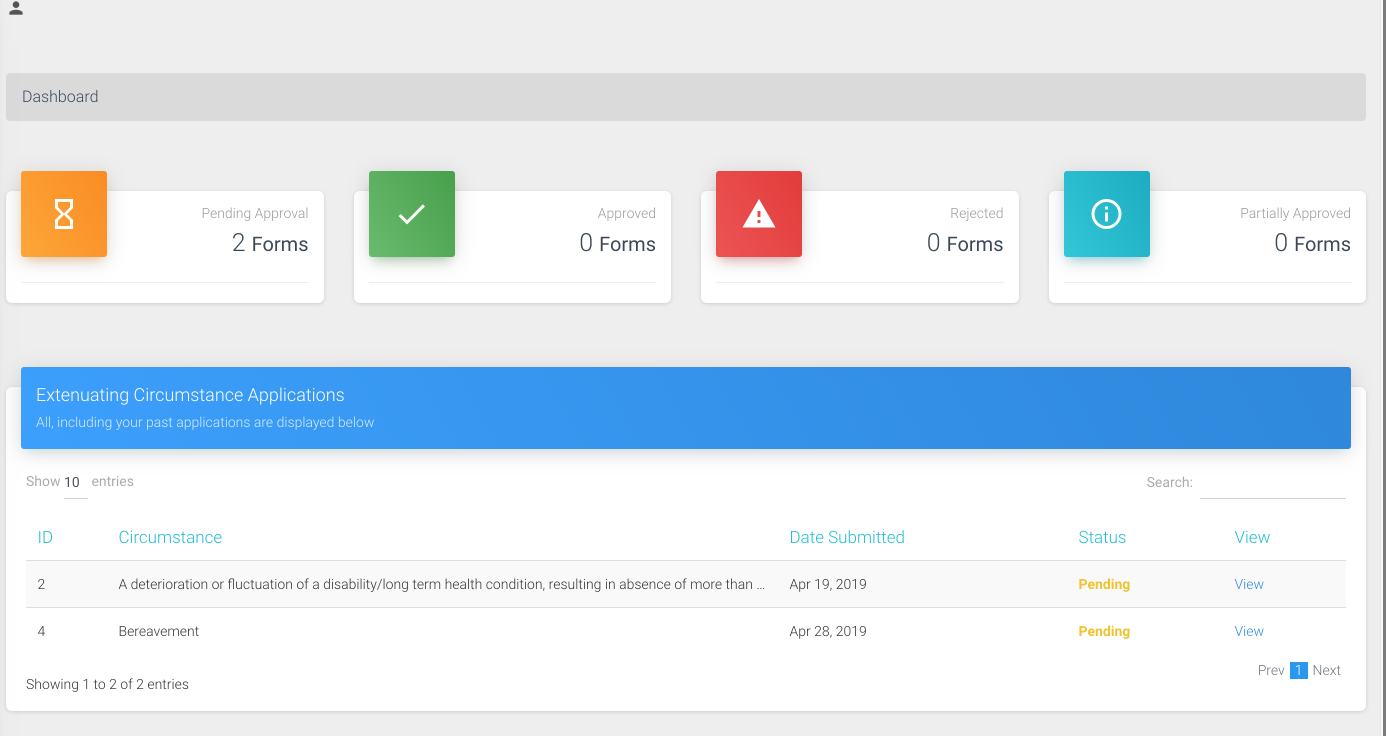
\includegraphics[scale=0.7]
        {images/dashboardimplement.png}
        \caption{\label{fig:dashboardimplement} Student Panel Dashboard}
      \end{figure}

\begin{figure}[H]
        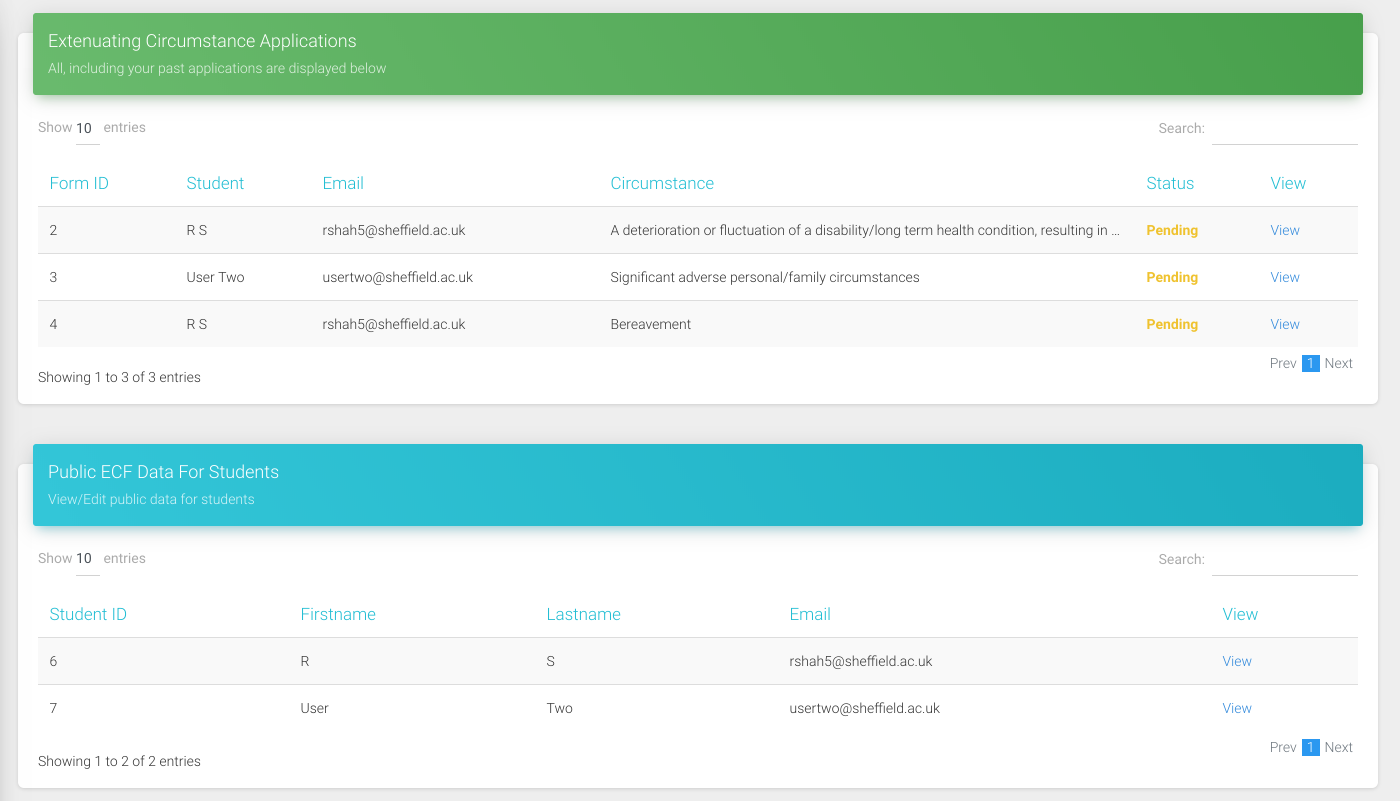
\includegraphics[scale=0.7]
        {images/secretarydashimplement.png}
        \caption{\label{fig:secretarydashimplement} Secretary Panel Dashboard}
      \end{figure}

\subsubsection{View Form} 

Student: The dashboard links each of the forms created to a view form page. This page retrieves data from the database based on the GET parameters(form ID) received when requesting the page. Interlinked data from the database is then retrieved based on the Form ID such as the \textit{User} who created it, the \textit{Files} uploaded under the form and lastly the \textit{Modules} affected. Each of these is stored in different tables as they share a one to many relationships. Apart from simply displaying the form data already submitted, there is an option triggered by the secretary which creates a new \textit{file uploader} at the top of the page allowing the student to upload more files. The file up-loader submits the new files as a POST form and saves based on the form ID. \\[4mm]

Secretary Panel: This page follows the same format as the student view form except for allowing the secretary to have control over editing the final status and action for each module and requesting more files. Each module is displayed in a table with individual buttons bringing up a \textit{pop-up} also known as \textit{Modal} in HTML5. The modal pop-ups then allow the secretary to change values for the \enquote{Action} and \enquote{Status} of the form. HTML drop-down allows us to display text as the displayed options while the back-end gets a \textit{value} which is stored into the database as an integer. This same value is automatically selected when displaying the current selection as it retrieves the integer from the database. A switch-case toggle was designed to allow the secretary to request more files from the student. When the switch is toggled, the database value for \enquote{requestfiles} is switched. This then displays the additional files up-loader as stated previously. The switch is called by a POST submit button with a \textit{name} attribute to differentiate between the different POST forms. Lastly, for ease of access, a \enquote{textarea} was created allowing direct change of the student's public data without having to open multiple tabs and make changes. This again uses a POST form with a different \enquote{name} attribute. Django views.py controls all the data received from the POST request and cleans the data ready to be saved into the database with the \textit{save()} function. Figures \ref{fig:secviewform} and \ref{fig:modal} shows PART of the view form page with and the popup which shows up when the edit button is clicked respectively.\\[4mm]

Scrutiny Panel: Since the scrutiny panel does not control the status directly on the portal, the view form page retrieves data from the database and displayed it with the use of HTML components. 

\begin{figure}[H]
        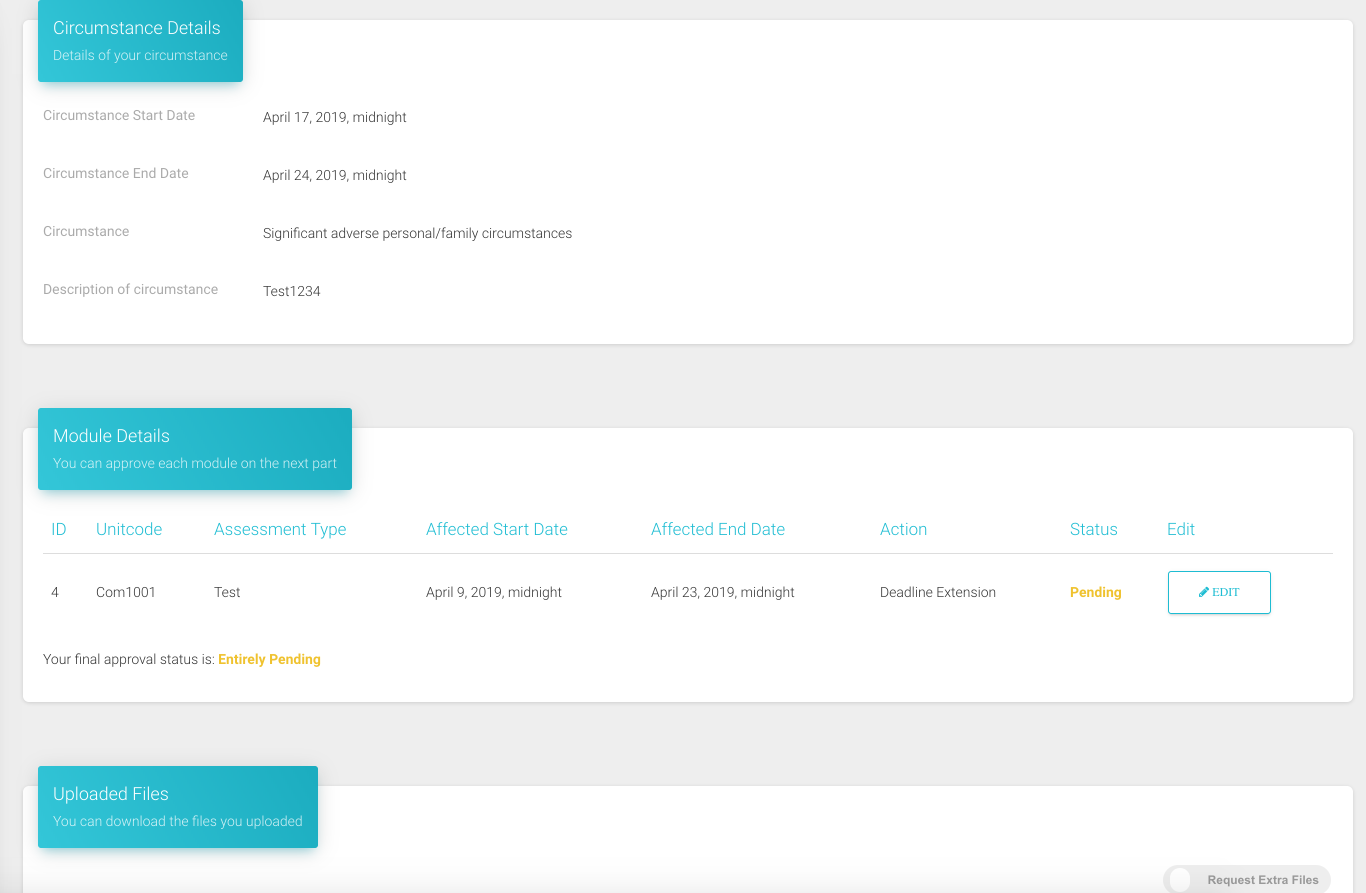
\includegraphics[scale=0.7]
        {images/secviewform.png}
        \caption{\label{fig:secviewform} PART of the Secretary Panel View Form}
      \end{figure}
      
\begin{figure}[H]
        \begin{center}
        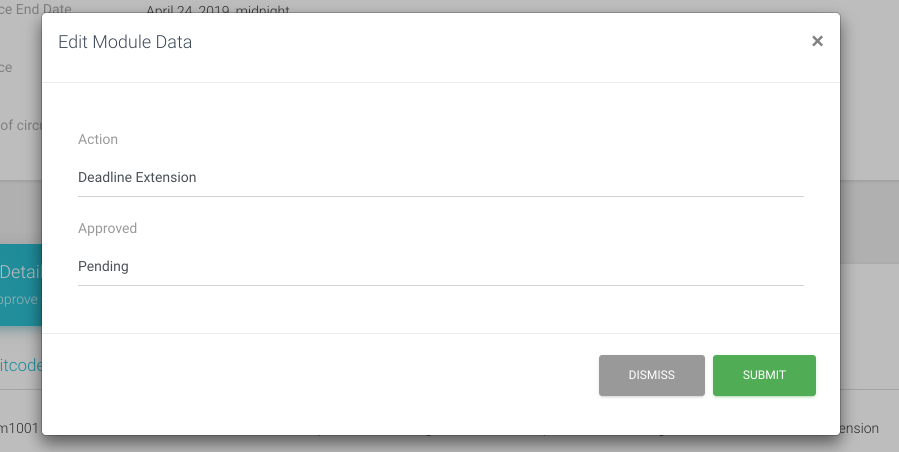
\includegraphics[scale=0.7]
        {images/modal.png}
        \caption{\label{fig:modal} Secretary Panel Edit Module Modal}
        \end{center}
      \end{figure}

\subsubsection{Profile Page} 
The profile page displays the current user's information. If the user is a student they can view their public data in a \textit{disabled} \textit{textarea}, this allows scrolling of long paragraphs without having to extend the page size. Users cannot change their email address as this would bring about issues of multiple sign-ups with different emails; hence the validation of only sheffield.ac.uk emails. A simple POST form on the page retrieves the values currently in the database and allows changing them after cleaning the new data. \textit{This includes: firstname; lastname; dob only.} Figure \ref{fig:profile} shows the student panel profile page with randomly generated text as the public data. 

\begin{figure}[H]
        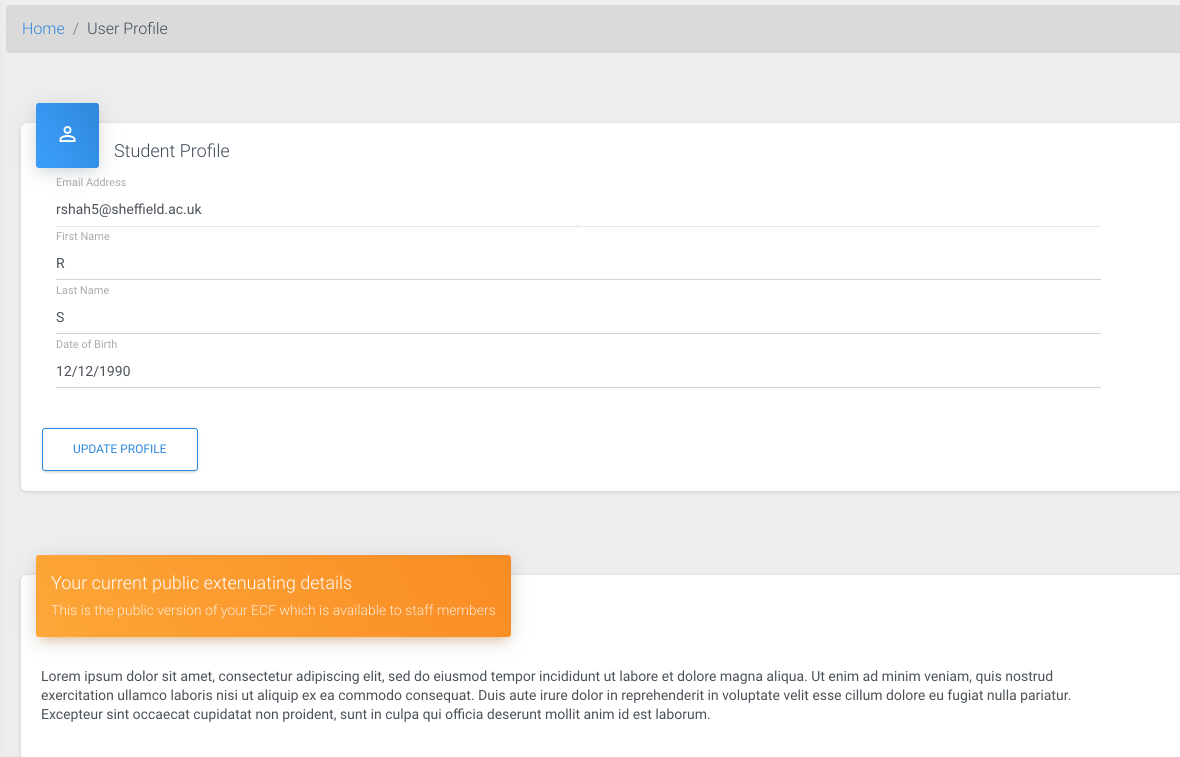
\includegraphics[scale=0.7]
        {images/profile.png}
        \caption{\label{fig:profile} Student Panel Profile Page}
      \end{figure}

\subsubsection{Student Record} 
Every user when registered is provided with a\textit{ eight digit random key} which can be used as a \textit{GET parameter} to access their public record. Only users who have the \textit{KEY} can access these records making it secure. This random key is stored in the database under \textit{User Profile} and has a unique schema which makes sure that two users do not have the same KEY. The public data again is displayed with a '\textit{textarea}' HTML component which is coded as mobile first. The purpose of using a random key is to avoid pattern detection (For example, using an email instead of a random key) and unauthorised access. Figure \ref{fig:studrecord} shows how the private link can be accessed and the data it would show. Since it is a \textit{textarea} HTML component, the data can be copied into a TXT when needed. \\[4mm]

Secretary Panel: Since only the secretary can give out the direct link to access the student's record, they also have access to regenerating the key. This is a safety feature to avoid unauthorised access. The regeneration uses the same principle of using Python's \textit{Random} package to generate an \textit{8 digit key} and replace it in the database. 

\begin{figure}[H]
        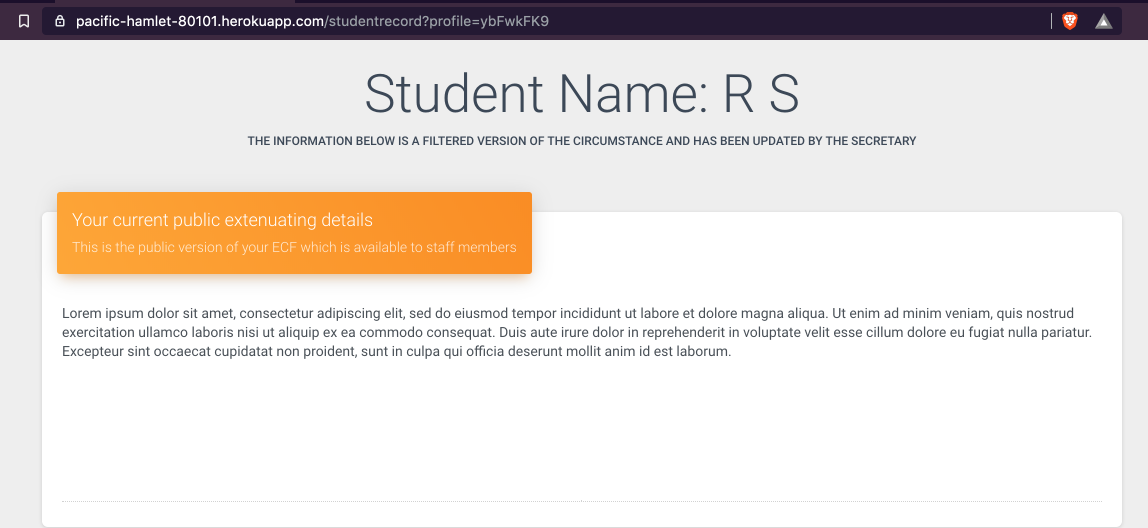
\includegraphics[scale=0.7]
        {images/studrecord.png}
        \caption{\label{fig:studrecord} Student Record Via Secret Link}
      \end{figure}

\subsubsection{Email Notifications} 
Email notification was created with the use of Gmail's SMTP services. Django has an inbuilt system which makes mailing and bulk mailing extremely easy. The SMTP details of the sender email can be set in the settings.py page which directly links to the Django mailer and with a simple \textit{sendMail} function we can send mail. To make debugging and later changes to the email text being sent, each message is stored as a TXT file which is called in the \textit{sendMail} function when required. For example, when a new user registers, a confirmation email is sent to the user using the \textit{sendMail} function and uses the data from NewUser.txt as the main message. Email notifications have been implemented for the following instances: New user registration; Password reset and confirmation of password change; Successful creation of extenuating circumstance form; Updated status of the form (Rejected/Approved); Requested additional files.


\end{document}
